%% question-9.tex
%%

%% ==============================
\subsection{Modélisation du concept de déclaration}
\label{sec:question9}
%% ==============================

Présentée à la figure \ref{fig:declaration}, la modélisation d'une \emph{Declaration} montre que celle-ci est comportée dans une \emph{Stratégie} et à 5 enfants : \emph{Variable}, \emph{Instruction}, \emph{Expression}, \emph{Module} et \emph{Paramètres}.

Un \emph{Module} comporte des variables et ces deux-ci ont un \emph{Type}. Le \emph{Module} prend également des \emph{Paramètres}.

\begin{figure}
	\centering
	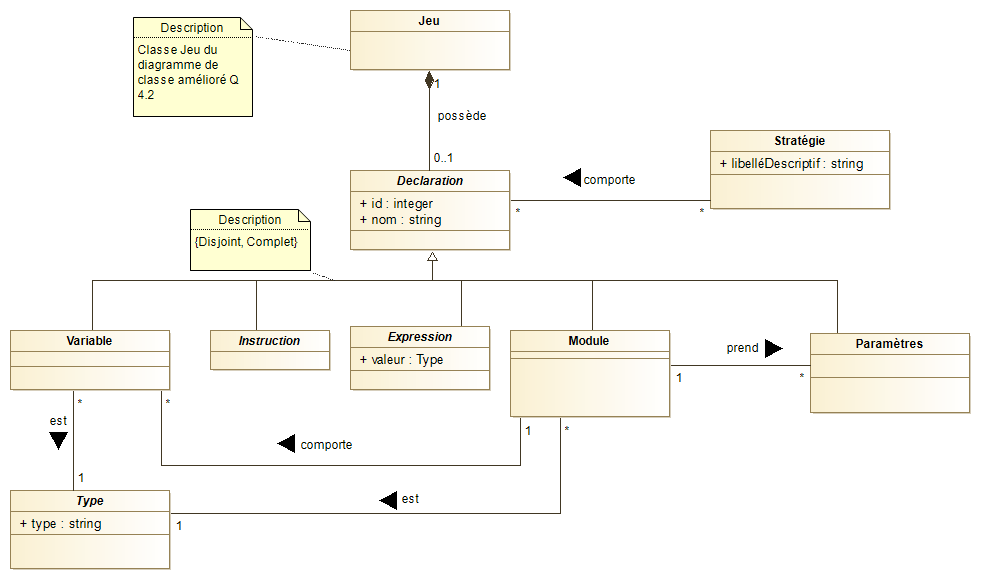
\includegraphics[width=500pt]{assets/class__Declaration}
	\caption{Diagramme de classe d'une déclaration}
	\label{fig:declaration}
\end{figure}
